% Financial Toolkit: 4-minute presentation (12 slides).
% Compile with pdfLaTeX (e.g. Overleaf). Figures in figures/ are redrawn at slide
% size by make_figures.py from the same code and data as examples/presentacion.ipynb.
%
% Fit rule: figures and the diagram are capped at a fraction of \textheight
% (keepaspectratio / adjustbox), so LaTeX shrinks them instead of letting them
% overflow; code slides keep at most 11 lines plus two lines of text.

\documentclass[aspectratio=169,10pt]{beamer}

\usepackage[utf8]{inputenc}
\usepackage[T1]{fontenc}
\usepackage{lmodern}
\usepackage[spanish,es-noshorthands]{babel}
\usepackage{booktabs}
\usepackage{listings}
\usepackage{adjustbox}
\usepackage{tikz}
\usetikzlibrary{positioning,fit,backgrounds,arrows.meta,babel}

\graphicspath{{figures/}}

% ---------------------------------------------------------------- Theme
\definecolor{ink}{HTML}{1F2A44}
\definecolor{accent}{HTML}{2E6BD8}
\definecolor{soft}{HTML}{EEF3FB}
\definecolor{good}{HTML}{2A8C55}
\definecolor{bad}{HTML}{C0392B}
\definecolor{muted}{HTML}{6B7280}

\usetheme{default}
\setbeamersize{text margin left=1cm, text margin right=1cm}
\setbeamertemplate{navigation symbols}{}
\setbeamercolor{frametitle}{fg=ink}
\setbeamercolor{title}{fg=ink}
\setbeamercolor{structure}{fg=accent}
\setbeamercolor{normal text}{fg=ink}
\setbeamerfont{frametitle}{series=\bfseries,size=\Large}
\setbeamertemplate{itemize items}{\color{accent}\textbullet}
\setbeamertemplate{footline}{%
  \leavevmode\hbox to \paperwidth{\hfill{\color{muted}\scriptsize Financial Toolkit
  \quad \insertframenumber/\inserttotalframenumber}\hspace{1em}}\vspace{0.5em}}
\setbeamertemplate{frametitle}{%
  \vspace{0.3em}\insertframetitle\par\vspace{-0.3em}%
  {\color{accent}\rule{2.5cm}{2pt}}}

\lstset{
  basicstyle=\ttfamily\footnotesize,
  columns=fullflexible,
  keepspaces=true,
  keywordstyle=\color{accent}\bfseries,
  stringstyle=\color{good},
  commentstyle=\color{muted}\itshape,
  backgroundcolor=\color{soft},
  frame=none,
  showstringspaces=false,
  language=Python,
  xleftmargin=0.4em,
  framexleftmargin=0.4em,
  aboveskip=0pt,
  belowskip=0pt,
}

\newcommand{\code}[1]{\texttt{\color{accent}#1}}

\title{Financial Toolkit}
\author{Hugo Ballestero \and Javier Arnanz \and Diego Antón}
\institute{Máster MIAX · BME Institute · Taller 1}
\date{10/11/2026}

\begin{document}

% ======================================================= 1. Title (~10 s)
\begin{frame}[plain]
  \titlepage
\end{frame}

% ===================================================== 2. What it is (~20 s)
\begin{frame}{Qué es}
  \begin{columns}[T]
    \begin{column}{0.36\textwidth}
      \begin{itemize}
        \item Librería de Python instalable: \code{financial\_toolkit}
        \item \textbf{Ingesta} desacoplada del \textbf{análisis}: todas las fuentes devuelven las mismas \emph{dataclasses}
        \item Añadir una API o un análisis no obliga a tocar el núcleo
      \end{itemize}
    \end{column}
    \begin{column}{0.60\textwidth}
      \small
      \begin{tabular}{@{}ll@{}}
        \toprule
        \textbf{Área} & \textbf{Fuentes / contenido} \\
        \midrule
        Acciones e índices & Yahoo Finance, FMP \\
        Criptomonedas      & Yahoo Finance, CoinGecko \\
        Fundamentales      & Los 3 estados financieros \\
        Tipos de interés   & EE.\,UU., BCE, Japón, BoE \\
        Macro              & FRED, World Bank \\
        Análisis           & Cartera, Monte Carlo, informe \\
        \bottomrule
      \end{tabular}
    \end{column}
  \end{columns}
\end{frame}

% ====================================================== 3. Data flow (~30 s)
\begin{frame}{Data flow}
  \begin{adjustbox}{max width=\textwidth, max totalheight=0.62\textheight, center}
  \begin{tikzpicture}[
      font=\footnotesize,
      box/.style={draw=accent, fill=white, rounded corners=2pt, align=center,
                  text width=2.6cm, minimum height=0.75cm, inner sep=2pt},
      obj/.style={box, fill=soft, font=\footnotesize\bfseries},
      group/.style={draw=muted!50, fill=muted!8, rounded corners=4pt, inner sep=6pt},
      glabel/.style={font=\small\bfseries, text=ink},
      arr/.style={-{Stealth[length=4pt]}, draw=ink!70, line width=0.6pt},
    ]
    % External APIs
    \node[box] (Y) at (0, 2.0)  {Yahoo Finance};
    \node[box] (F) at (0, 1.0)  {FMP};
    \node[box] (C) at (0, 0.0)  {CoinGecko};
    \node[box] (B) at (0,-1.0)  {US Treasury / ECB\\ Japan / BoE};
    \node[box] (M) at (0,-2.2)  {FRED / World Bank};
    % Ingestion layer
    \node[box] (CL) at (3.6, 1.6) {\texttt{clean\_prices}};
    \node[box] (AF) at (3.6, 0.3) {\texttt{AssetFetcher}\\\texttt{.get\_many}};
    \node[box] (BN) at (3.6,-1.0) {\texttt{BondNormalizer}};
    \node[box] (MF) at (3.6,-2.2) {\texttt{MacroFetcher}};
    % Standard objects
    \node[obj] (A)  at (7.2, 1.6) {Stock / Index /\\ Cryptocurrency\\ + PriceSeries};
    \node[obj] (BO) at (7.2,-1.0) {Bond};
    \node[obj] (MS) at (7.2,-2.2) {MacroSeries};
    % Analysis layer
    \node[box] (P)  at (10.8, 1.6) {\textbf{Portfolio}};
    \node[box] (MC) at (10.8, 0.3) {MonteCarloResult};
    \node[box] (R)  at (10.8,-1.0) {\texttt{report} (Markdown)};
    \node[box] (PL) at (10.8,-2.2) {\texttt{plots\_report}};
    \coordinate (bypass) at ([xshift=0.45cm]P.east);
    \coordinate (top) at (Y.north);
    \coordinate (bot) at (M.south);

    % All four groups share the same top and bottom edge.
    \begin{scope}[on background layer]
      \node[group, fit=(Y)(M)]                                (G1) {};
      \node[group, fit=(CL)(MF)(top -| CL)(bot -| CL)]        (G2) {};
      \node[group, fit=(A)(MS)(top -| A)(bot -| A)]           (G3) {};
      \node[group, fit=(P)(PL)(bypass)(top -| P)(bot -| P)]   (G4) {};
    \end{scope}
    \node[glabel, above=1pt of G1] {External APIs};
    \node[glabel, above=1pt of G2] {Ingestion layer};
    \node[glabel, above=1pt of G3] {Standard objects};
    \node[glabel, above=1pt of G4] {Analysis layer};

    % Arrows: the same edges as the README flowchart
    \foreach \s in {Y,F,C,B} \draw[arr] (\s.east) -- (AF.west);
    \draw[arr] (AF) -- (CL);
    \draw[arr] (AF) -- (BN);
    \draw[arr] (CL) -- (A);
    \draw[arr] (BN) -- (BO);
    \draw[arr] (M)  -- (MF);
    \draw[arr] (MF) -- (MS);
    \draw[arr] (A)  -- (P);
    \draw[arr] (P)  -- (MC);
    \draw[arr] (MC) -- (R);
    \draw[arr] (P.east) -- (bypass) |- (R.east);
    \draw[arr] (bypass) |- (PL.east);
  \end{tikzpicture}
  \end{adjustbox}

  \vspace{0.4em}
  \centering
  {\small El análisis solo conoce los objetos estándar, \textbf{nunca la respuesta cruda de una API}.}
\end{frame}

% ===================================== 4. Code: download N assets (~25 s)
\begin{frame}[fragile]{Código: N activos de cualquier fuente en una llamada}
\begin{lstlisting}
requests = [
    {"type": "stock", "api": "yfinance", "symbol": "AAPL"},
    {"type": "stock", "api": "fmp", "symbol": "MSFT"},
    {"type": "crypto", "api": "coingecko", "symbol": "bitcoin"},
    {"type": "index", "api": "yfinance", "symbol": "^GSPC"},
    {"type": "bond", "api": "bce", "symbol": "EU10Y"},
]
fetcher = AssetFetcher()
assets = fetcher.get_many(requests, start="2023-01-03", end="2025-10-31")
fetcher.cleaning_reports["AAPL"]   # CleaningReport for each asset
\end{lstlisting}
  \vspace{0.5em}
  \small
  Yahoo y FMP devuelven la \textbf{misma clase} \code{Stock} (diferencia media de cierre: 0,0009\,\%), y CoinGecko devuelve \code{Cryptocurrency} con sus \code{Tokenomics}.
\end{frame}

% ===================================== 5. Code: get_many inside (~30 s)
\begin{frame}[fragile]{Código: qué hace \texttt{get\_many()} por dentro (simplificado)}
\begin{lstlisting}
fetchers = {                                  # 10 (type, api) combinations
    ("stock", "yfinance"): self.yahoo.get_stock,
    ("crypto", "coingecko"): self.coingecko.get_crypto,
    ("bond", "bce"): self.bce.get_data,
}
for request in requests:
    asset = fetchers[(kind, api)](**parameters)
    if kind == "bond":
        asset = self.bond_normalizer.normalize(data=asset, ...)
    else:
        prices, report = clean_prices(self._trim(asset, start, end).price)
\end{lstlisting}
  \vspace{0.5em}
  \small
  \begin{itemize}
    \item \textbf{Añadir una API = añadir una entrada} al diccionario: el resto del código no cambia
    \item Las acciones, índices y criptos se recortan al periodo y se limpian; los bonos se normalizan a \code{Bond}
  \end{itemize}
\end{frame}

% ============================ 6. Code: PriceSeries, fundamentals, macro (~25 s)
\begin{frame}[fragile]{Código: PriceSeries, fundamentales y macro}
\begin{lstlisting}
prices = aapl.price                               # PriceSeries
prices.annual_return, prices.annual_volatility    # 27.8 %, 25.9 %: computed on creation
prices.sma(50), prices.ema(20), prices.bollinger_bands()
prices.rsi(), prices.macd(), prices.max_drawdown()          # drawdown -33.4 %

aapl.company.fundamentals.analyze_income_statement()  # margins, growth, warnings

macro = MacroFetcher()
bill = macro.get_macro_series("DTB3", source="FRED", start=START, end=END)
risk_free = float(bill.data.dropna().iloc[-1]) / 100     # 3.73 %
\end{lstlisting}
  \vspace{0.5em}
  \small
  Los estadísticos se calculan \textbf{al crear el objeto}; los indicadores son métodos. El tipo libre de riesgo de FRED alimenta después el Sharpe.
\end{frame}

% ==================================== 7. Charts: indicators and bonds (~15 s)
\begin{frame}{Gráficos: indicadores de AAPL y bonos a 10 años}
  \centering
  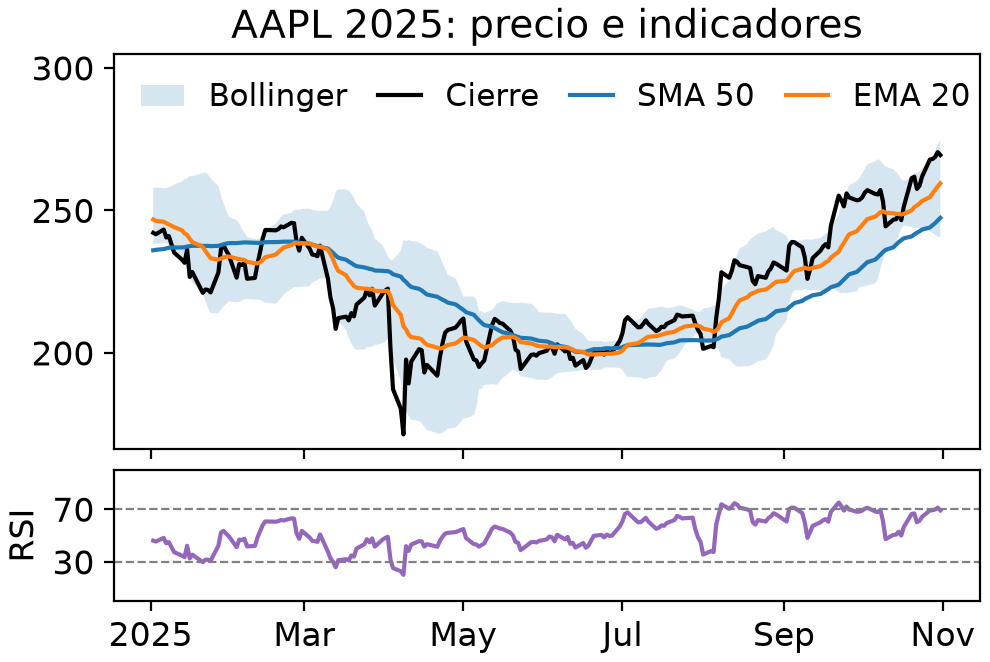
\includegraphics[width=0.48\textwidth,height=0.62\textheight,keepaspectratio]{aapl_indicators}\hfill
  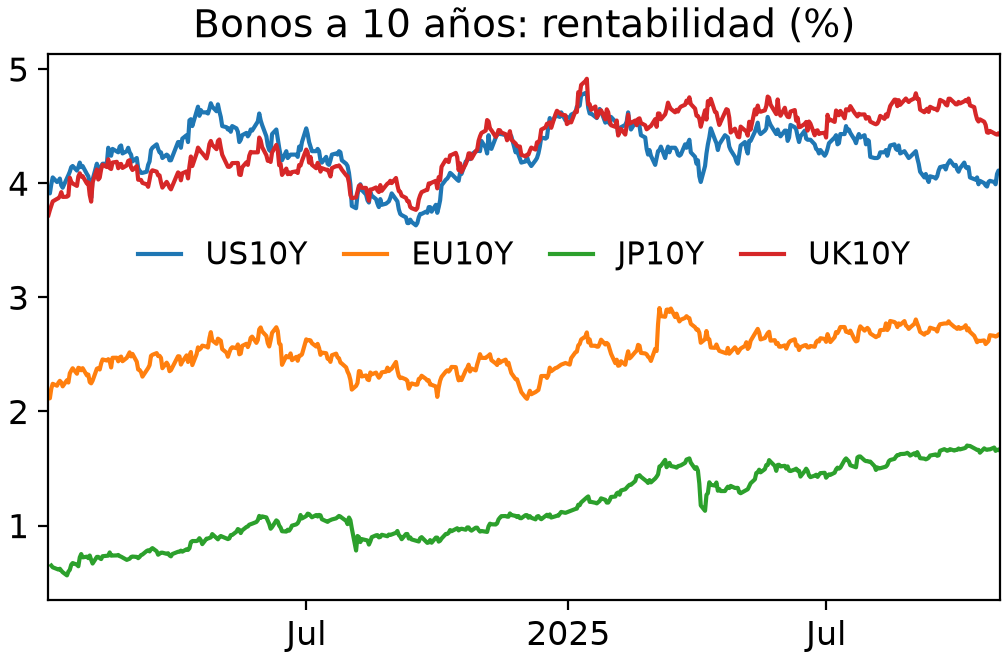
\includegraphics[width=0.48\textwidth,height=0.62\textheight,keepaspectratio]{bonds_10y}
\end{frame}

% ===================================== 8. Code: cleaning and validation (~30 s)
\begin{frame}[fragile]{Código: datos honestos y validación estricta}
\begin{lstlisting}
clean, report = clean_prices(dirty_series)       # 2 missing closes + an unadjusted split
# CleaningReport(n_input=250, n_output=248, ..., missing=2, outliers=1)
clean_prices(too_dirty_series)                    # 10 % of the closes missing
# ValueError: missing closes must be at most 5%, got 10.00% (25 of 250)

Portfolio.from_weights([san_eur], [1.0], 10_000, date)
# ValueError: Convert asset prices to USD before trading
Portfolio.from_weights([bond], [1.0], 10_000, START)
# TypeError: Invalid asset type
\end{lstlisting}
  \vspace{0.5em}
  \small
  \begin{itemize}
    \item Los cierres inválidos \textbf{se eliminan, no se rellenan}; los outliers \textbf{se cuentan, no se tocan}
    \item Mejor un \textbf{error claro} que una métrica falsa
  \end{itemize}
\end{frame}

% ===================================== 9. Code: portfolio and Monte Carlo (~30 s)
\begin{frame}[fragile]{Código: cartera y Monte Carlo}
\begin{lstlisting}
weights = {"AAPL": 0.25, "MSFT": 0.25, "SAN": 0.15, "IEF": 0.20, "BTC-USD": 0.15}
portfolio = Portfolio.from_weights([aapl, msft, san, ief, btc], weights, 10_000, START)
portfolio.buy(aapl, 10, "2024-01-03")            # paid with cash
portfolio.deposit(5_000, "2024-06-03")           # external flow, not a gain
portfolio.rebalance([aapl, msft, san, ief, btc], weights, "2025-01-02")

simulation = portfolio.monte_carlo(10_000, years=1, seed=42)
stress = portfolio.monte_carlo(10_000, years=1, annual_return=0.03, annual_volatility=0.35)
portfolio.report(risk_free=risk_free, monte_carlo=simulation)    # Markdown
\end{lstlisting}
  \vspace{0.6em}
  \centering
  \footnotesize
  \begin{tabular}{@{}cccccc@{}}
    \toprule
    Aportado & Valor final & TWR & Volatilidad & Sharpe & Máx. drawdown \\
    \midrule
    15.000 USD & \textbf{37.198 USD} & 195,7\,\% & 16,8\,\% & \textbf{2,04} & $-$14,2\,\% \\
    \bottomrule
  \end{tabular}
\end{frame}

% ===================================== 10. Chart: Monte Carlo (~20 s)
\begin{frame}{Gráfico: Monte Carlo a 1 año}
  \centering
  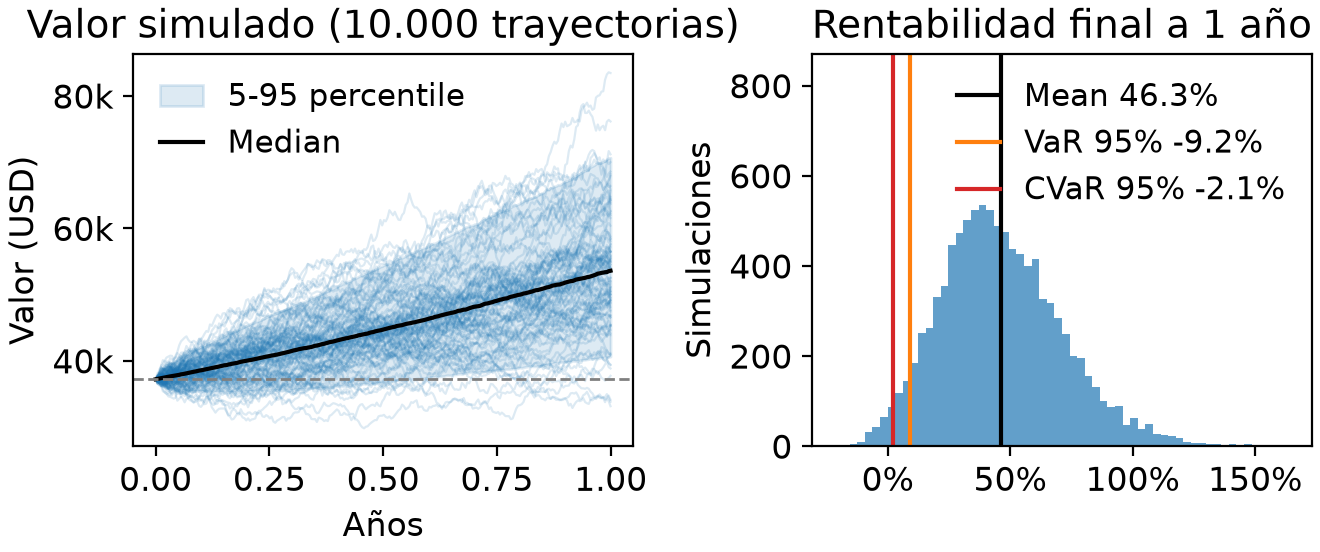
\includegraphics[width=\textwidth,height=0.42\textheight,keepaspectratio]{monte_carlo}

  \vspace{0.5em}
  \footnotesize
  \begin{tabular}{@{}lrrr@{}}
    \toprule
                       & Histórico & Estrés 3\,\%/35\,\% & Solo BTC \\
    \midrule
    Rentabilidad media & 46,3\,\% & 9,9\,\%  & 119,4\,\% \\
    Mediana            & 44,1\,\% & 3,0\,\%  & 94,5\,\% \\
    Prob. de pérdida   & 1,6\,\%  & \textbf{46,7\,\%} & 8,4\,\% \\
    \bottomrule
  \end{tabular}
\end{frame}

% ===================================== 11. Chart: plots_report (~15 s)
\begin{frame}{Gráfico: \texttt{plots\_report()}}
  \centering
  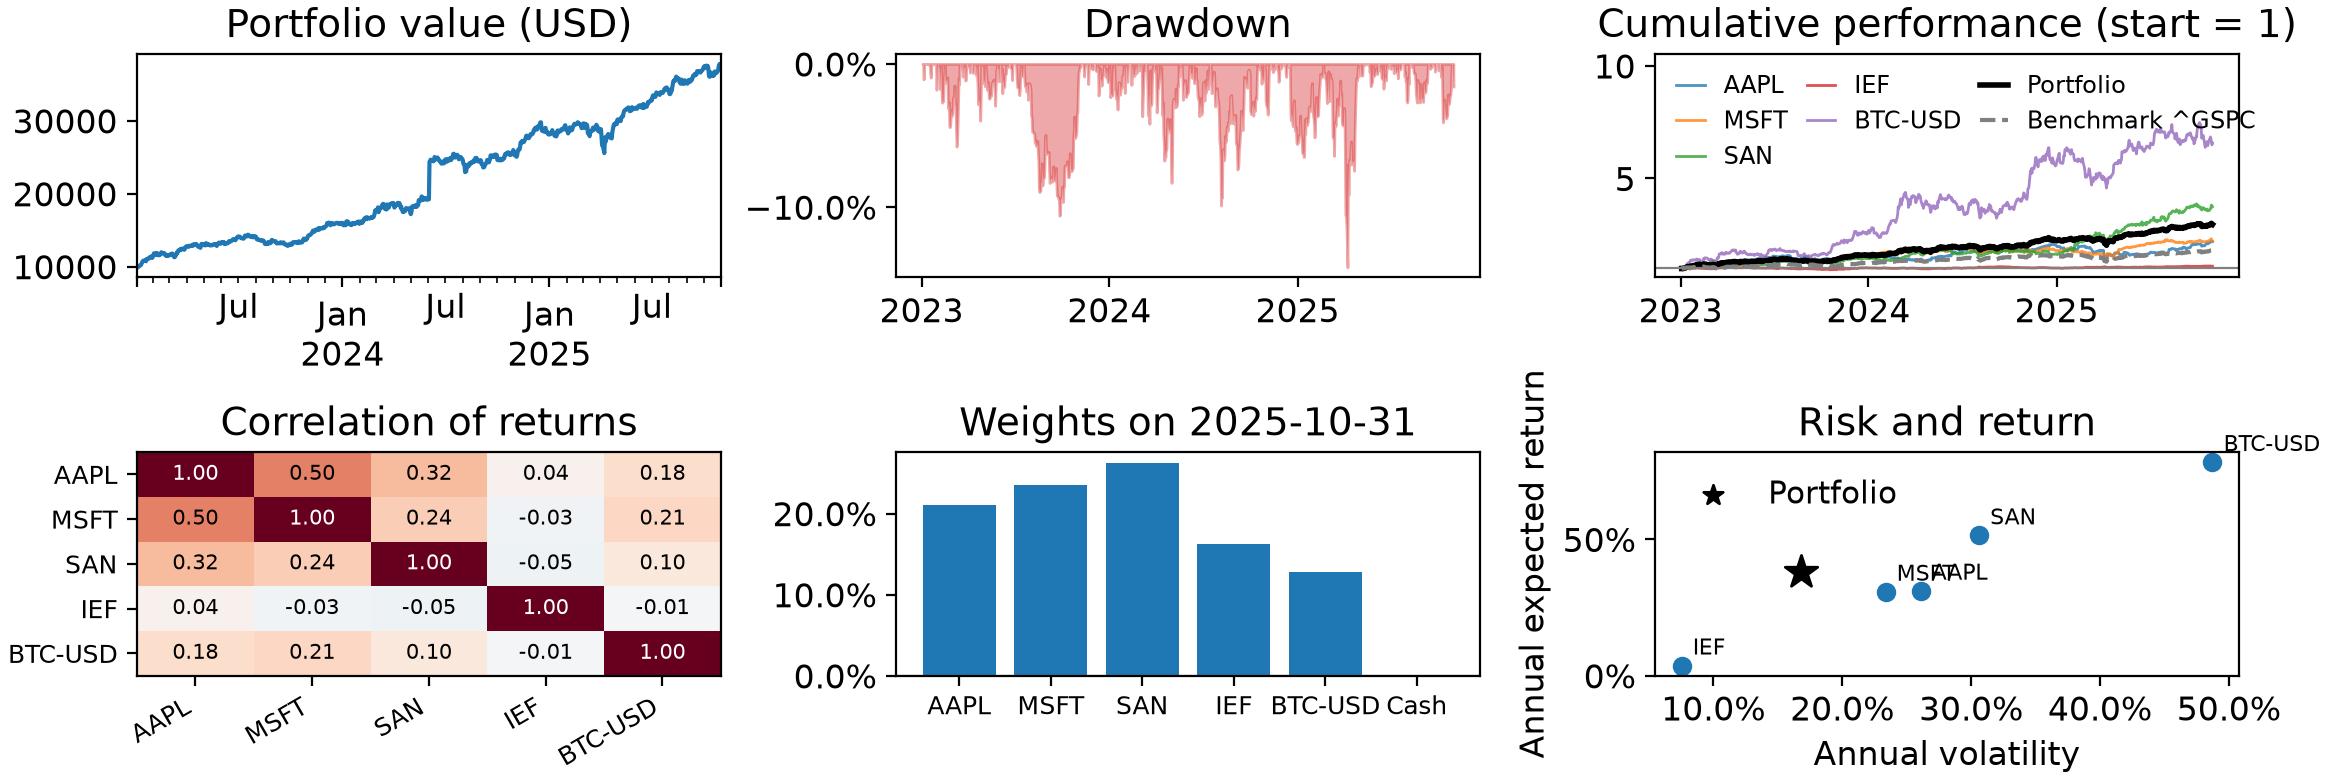
\includegraphics[width=\textwidth,height=0.66\textheight,keepaspectratio]{plots_report}
\end{frame}

% ===================================== 12. Conclusions (~20 s)
\begin{frame}{Conclusiones}
  \begin{itemize}
    \setlength{\itemsep}{0.6em}
    \item \textbf{Diseño en capas}: añadir una API o un análisis no obliga a tocar el resto
    \item \textbf{Salida estandarizada}: Yahoo, FMP, CoinGecko y 4 bancos centrales producen los mismos objetos
    \item \textbf{Datos honestos}: no se rellenan precios, los outliers se avisan y las métricas usan solo fechas observadas
    \item \textbf{Validación estricta}: errores claros antes que números falsos
  \end{itemize}
  \vspace{1.2em}
  \centering {\Large\color{accent}\textbf{¡Gracias!}}
\end{frame}

\end{document}
